\chapter{Results}

Studies of several emission peaks of neutral Ba in SXe are discussed in \ref{sec:fluorescence}.  Bleaching of these peaks is discussed in detail in \ref{sec:bleaching}.  Imaging of Ba fluorescence in a focused laser region is discussed in \ref{imaging}, with the ultimate achievement of imaging at the single atom level using the 619-nm fluorescence peak.  Candidate fluorescence peaks of Ba\textsuperscript{+} in SXe are reported in \ref{sec:BaPlus}.

\section{Fluorescence of Ba in SXe}
\label{sec:fluorescence}

Deposits of Ba in SXe absorb primarily between 540~nm and 570~nm \cite{Mong2015,Brian,Shon}.  An absorption spectrum, obtained by observing absorption of white light by a large Ba deposit at 11~K, is shown in Fig. \ref{fig:BaAbs}, along with an example emission spectrum.  Significant broadening, as well as a 4-nm redshift  of the central peak, occur relative to the vacuum absorption value of 553.5~nm.

Several red-shifted emission peaks are observed and attributed to Ba atoms occupying different matrix sites in the SXe.

\begin{figure} %[H]
        \centering
                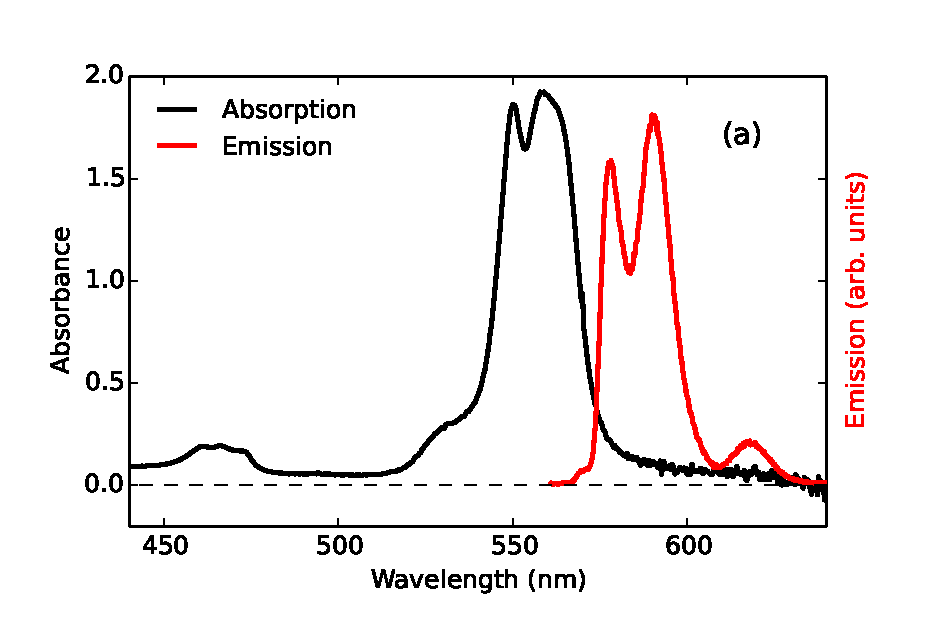
\includegraphics[width=.7\textwidth]{figures/BaAbs_fromBaSpec.eps}
                \caption{\color{red}Get rid of the (a).  Probably need to just edit screenshot with paint.  \cite{Mong2015}}
\label{fig:BaAbs}
\end{figure}

excitspec of 50~K [fig of all, including r110 of 619]... and 10~K?  representative spectra showing all the different peaks

leak rate dependence?

\subsection{Identifying Peaks as Ba in SXe}
\label{subsec:peakIdentify}

\emph{\color{gray}This section was claimed in Ba getter section of Chapter 3 to talk about getter use in identifying 619.}

\subsection{Temperature/annealing}

\section{Bleaching}
\label{sec:bleaching}

({\color{red}do a correction on p-meter sensitive area and on p-meter quantum efficiency, and also a spherical aberation correction for power, though that may not matter for the defocused studies.})

590 etc, model fit (see results intro paragraph)

\begin{figure} %[H]
        \centering
                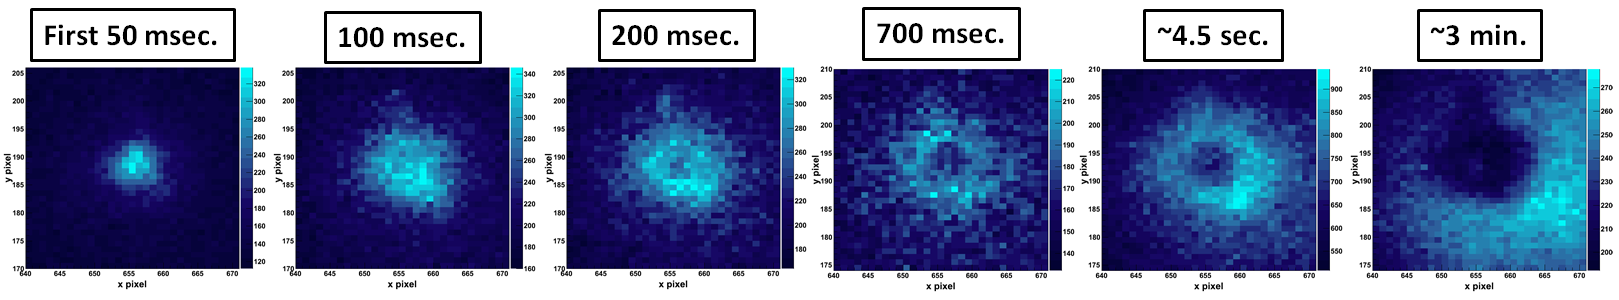
\includegraphics[width=.9\textwidth]{figures/hole_bleach_590.png}
                \caption{}
\label{fig:testfig}
\end{figure}

619, with the changes in time and I

\section{Imaging}
\label{imaging}

\subsection{Imaging 577- and 591-nm peaks}

\subsection{Imaging 619-nm peak}

\begin{figure} %[H]
        \centering
                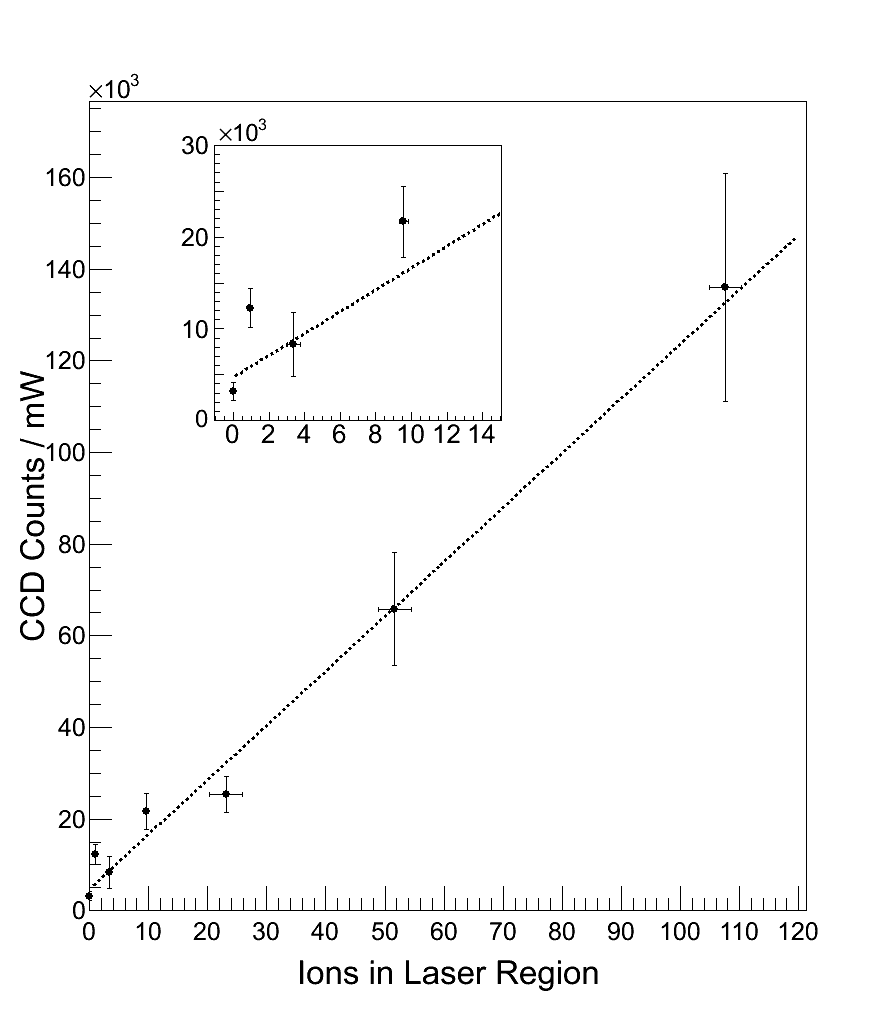
\includegraphics[width=.7\textwidth]{figures/fitgrouped_20150807_20150916_inset.png}
                \caption{Combined 2015-08-07 and 2015-09-16 with statistical errors.  \emph{\color{gray}Move y-axis title over.}}
\label{fig:lin}
\end{figure}

\section{Candidate Ba\textsuperscript{+} Lines}
\label{sec:BaPlus}